\documentclass[12pt]{article}
%Gummi|065|=)
\usepackage{amsmath, amsfonts, amssymb}
\usepackage[margin=0.5in]{geometry}
\usepackage{xcolor}
%\usepackage{graphicx}
%\usepackage{graphicx}
\newcommand{\off}[1]{}
\DeclareMathSizes{20}{30}{21}{18}

\newcommand{\myhrule}{}

\newcommand{\dash}{
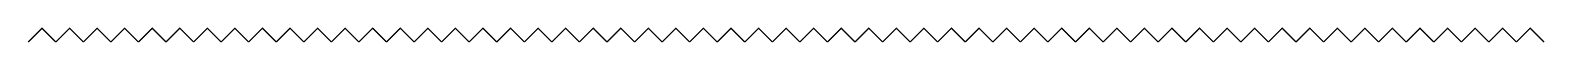
\begin{tikzpicture}[scale=0.35]
\foreach \x in {1,...,55}{
	\draw (\x,-0.25)--(\x+0.5,0.25)--(\x+1,-0.25);
}
\end{tikzpicture}
}

\usepackage{tikz}

\title{\textbf{ Examples: Halasz Inequality}}
\author{John D Mangual}
\date{}
\begin{document}

\fontfamily{qag}\selectfont \fontsize{25}{30}\selectfont

\maketitle

\noindent In the nice paper of Radiziwill and Motomaki they talk about the ``pretentious number theory".  Two {\color{blue}multiplicative} functions pretend as measured by:
$$ \mathbb{D}(f,g; x)^2 = \sum_{p \leq x} \frac{1 - \mathrm{Re}\big[\;f(p)\overline{g(p)}\;\big]}{p} $$
and this distance measure satisfies triangle inequality
$$ \mathbb{D}(f,h; x) \leq
\mathbb{D}(f,g; x) +\mathbb{D}(g,h; x) $$
however this is \textbf{not} a metric since this distince function is sometimes negative.\footnote{Somewhat like the Kullback-Liebler divergence from information theory.  Except - there is no triangle inequality; could be the Fisher information metric?} \\ \\
This pretending metric $\mathbb{D}$ is defined for any functions $f,g$ or $h: \mathbb{N} \to \{ z \in \mathbb{C}: |z| \leq 1 \}$ mapping to the unit disk.

\newpage

\noindent Granville and Soundarajan are usually looking to find if a multiplicative function is pretending to be something it's not. 
$$ \mathbb{D}\Big( \mu(p) , p^{it} ; x\Big)^2
= \sum_{p \leq x} \frac{1 -  \cos \big(t\, \log p\big) }{p}$$
Here $\mu(x)$ is the \textbf{M\"{o}bius function} which is multiplicative on $\mathbb{N}$ and $\mu(p) = -1$ for all primes. \\ \\
This distance is a {\color{red!50!white} trigonometric series} over $t$ and we can ask about the miminum value, for $-T < t < T$. Call it $M$.\\ \\
The \textbf{Halasz-Montgomery-Tenenbaum} theorem says
$$ \frac{1}{x} \Big| \sum_{n \leq x} f(n)\Big|
\ll (1+M) \, e^{-M} + O\left( \frac{1}{\sqrt{T}}\right) $$
$\log p$ is an interesting choice of frequencies 
\begin{itemize}
\item $\log n$ is not equidistributed mod $1$ (these are the numbers after the decimal point)  yet
\item $\displaystyle \frac{1}{N} \sum_{n \leq N} e^{2\pi i \log n} \to 0 $ we conclude $e^{2\pi i \, \log n} \to 0 $
\end{itemize}

\newpage

\noindent Weyl's Theorem (Satz 21) says:
\begin{quotation}
Let $\lambda_1, \lambda_2, \dots $ be a sequence of real numbers. If we can find two numbers $c, \epsilon$ such that $$ \big| 
\lambda_{n + \frac{n}{(\log n)^{1+\epsilon}}} - \lambda_n\big| \geq c $$
Then for $x$ away from a set of measure\footnote{the German says ``mass"} 0 the sequence
$$ \lambda_1 x \, \lambda_2 x \, \dots $$
is equidistributed mod $0$.
\end{quotation}
This is a very funny condition for Weyl to put.
$$ \lambda_{n\big( 1 + \frac{1}{(\log n)^{1+\epsilon}}\big)} - \lambda_n \geq c$$
E.g. $\lambda_n = a^n$ with $a > 1$.  Hardy write this the conclusion as\footnote{without ever saying $N \to \infty$ or somthing precise like that} an average tending to zero:
$$ \frac{1}{N}\sum_{n=1}^N e^{\lambda_n x} = o(1)$$
and that $\{\lambda_n x\}$ is equidistributed \textbf{except} at set of measure 0, i.e. ``never". \\ \\
E.g. $\lambda_n = \log n$ we got $\frac{1}{N}\sum e^{2\pi i \, x \log n}  = O(1)$ a.e.\footnote{``almost everywhere" I think $x = 1$ works, but maybe you need $x = 1.00001$ or something.  j/k $x = 1$ works.}


\newpage

\noindent I got caught up on this reading Kupers and Neiderreiter.  One has this result.
$$ \frac{1}{N}\sum e^{2\pi i \, x_n}= o(1) \longrightarrow n \big|x_{n+1}-x_n \big| \to \infty$$
Then if $x_n = \log n$ are function does not grow fast enough:
$$ n (\log (n+1) - \log n) \approx n \times \frac{1}{n} = 1 < \infty $$
and this sequence is known to diverge.
$$ \frac{1}{N}\sum_{n=1}^N e^{2\pi i \, \log n } \not \to 0 \text{ it is }O(1)$$
This average spirals around $0$ forever.   To prove this theorem Kuipers-Neiderreiter cite a ``well-known Tauberian Theorem" \\ \\
If $n |x_{n+1}-x_n| = \infty $ then by triangle inequality and $1+x < e^x$ we have:
$$ |e^{2\pi i x_{n+1}}- e^{2\pi i x_n} |\leq 2\pi |x_{n+1}-x_n| = O(1/n) $$
and we know the Weyl average must be zero
$$ \lim_{N \to \infty }  \frac{1}{N} \sum_{n=1}^N e^{2\pi i x_n} = 0$$
a well-known theorem shows $e^{2\pi i x_n} \to 0$.

\newpage

\noindent The well-known theorem could be:
$$ a_n = O( \tfrac{1}{N}) \text{ and }\lim_{x \to 1} \sum_{n=0}^\infty a_n x^n = s \longrightarrow \sum_{n=0}^\infty a_n = s $$
this is equivalent to the prime number theorem.  Example we might consider are:
\begin{itemize}
\item $a_n = e^{2\pi i \, x_{n+1}} - e^{2\pi i \, x_n } $ and $|x_{n+1}-x_n| = O(\tfrac{1}{n})$
\item $a_n = e^{2\pi i \, \log(n+1)} - e^{2\pi i \, \log n }  $ (and $\tfrac{1}{N} \sum e^{2\pi i \, \log n} \neq 0$)
\item $a_n = \Lambda(n)$ (the van Mangoldt function)
\end{itemize}
There is lots of trigonometry here but the shape not very geometrical and awfully hard to visualize.  \\ \\
\textbf{Halasz Theorem}  (again)
$$ \frac{1}{x}\big| \sum_{n \leq x} f(n) \big| \ll (1+M)e^{-M} + O(1/\sqrt{T})  $$ 
if we solve the trigonometry problem of finding the minimum for $|t| < T$.
 $$M = \mathbb{D}(f, p^{it}; x) = \sum_{p < x} \frac{1 - f(p) p^{-it}}{p} $$ 

\newpage

\fontfamily{qag}\selectfont \fontsize{12}{10}\selectfont


\begin{thebibliography}{}

\item Kaisa Matom\"{a}ki, Maksym Radziwi\l\l{} \textbf{Multiplicative functions in short intervals} \texttt{arXiv:1501.04585}

\item Andrew Granville , Kannan Soundararajan \textbf{Decay of mean-values of Multiplicative Functions} \texttt{arXiv:math/9911246}

\item Hermann Weyl \textbf{\"{U}ber die Gleichverteilung von Zahlen mod. Eins}. Mathematische Annalen 77 (3): 313-352 (1916)

\item \texttt{http://math.stackexchange.com/q/1940261/4997}

\item Kuipers, Niederreiter \textbf{Uniform Distribution of Sequences} Dover, 2006.

\item Antoni Zygmund \textbf{Trigonometric Series}, Cambridge Mathematical Library.  CUP, 2003.


\end{thebibliography}



\end{document}